\section{Experimental Setup}

All experiments were conducted on antibiotic-specific datasets built from the same shared genotype-phenotype cohort. The same phenotype-cleaning logic, genotype normalization logic, and class-count thresholds were used across all scopes so that differences in performance can be attributed to the determinant-connection strategy rather than to a changing cohort.

The final experiment set contains 14 antibiotics: amoxicillin-clavulanic acid, ampicillin, cefoxitin, ceftiofur, ceftriaxone, chloramphenicol, ciprofloxacin, gentamicin, kanamycin, nalidixic acid, streptomycin, sulfisoxazole, tetracycline, and trimethoprim-sulfamethoxazole.

The machine-learning comparison includes three settings, namely \textbf{Strict ML}, \textbf{Broad ML}, and \textbf{All ML}, while the direct genotype-to-phenotype reference baselines are \textbf{Strict rule-based} and \textbf{Broad rule-based}. This design is more informative than a generic comparison of many classifiers because it isolates the effect of biological connection scope and makes it possible to distinguish between gain from using broader genotype evidence and gain from replacing direct scope-based rules with learned combination logic.

\section{Comparative Performance}

\subsection{Average performance across methods}

Table~\ref{tab:method-average-metrics} summarizes the average performance of the five main method settings across the 14 antibiotics. For the machine-learning settings, the values come from the final scope-specific outputs produced by the pipeline. Rule-based averages are retained as the direct deterministic reference.

\begin{table}[H]
\centering
\caption{Average performance across antibiotics}
\label{tab:method-average-metrics}
\small
\begin{tabular}{lccccc}
\toprule
Method & Accuracy & Precision & Recall & ROC-AUC & Avg. zero rows \\
\midrule
Strict rule-based & 0.861 & 0.655 & 0.704 & --    & 4461.1 \\
Broad rule-based  & 0.839 & 0.648 & 0.987 & --    & 3790.5 \\
Strict ML         & 0.822 & 0.744 & 0.860 & 0.842 & 4461.1 \\
Broad ML          & 0.988 & 0.972 & 0.975 & 0.984 & 3790.5 \\
All ML            & 0.987 & 0.966 & 0.974 & 0.988 & 0.0 \\
\bottomrule
\end{tabular}
\end{table}

Several observations follow directly from Table~\ref{tab:method-average-metrics}. First, the machine-learning settings dominate the overall comparison. Both \textit{broad ML} and \textit{all ML} achieve average recall near \(0.974\) or higher and average accuracy near \(0.99\), whereas \textit{strict ML} remains much weaker because the narrow scope leaves too many isolates with no determinant evidence.

Second, \textit{broad ML} and \textit{all ML} differ in an important way. \textit{Broad ML} has slightly stronger average recall and precision, while \textit{all ML} has the highest average ROC-AUC and removes the zero-feature problem completely. This means the advantage of \textit{all} is not that it wins every average metric; rather, its advantage is that it provides the widest usable feature coverage and the strongest overall separability.

Third, the rule-based baselines clarify why machine learning is valuable. \textit{Broad rule-based} achieves extremely high recall on average, but with weak precision, which indicates that direct within-class determinant matching can recover many resistant isolates at the cost of overcalling resistance.

\subsection{Performance pattern of the three ML scopes}

The machine-learning scopes show a consistent progression from narrow to wide evidence usage. \textbf{Strict ML} is the narrow biological reference. It uses the smallest average feature set (\(\approx 32.6\) features per antibiotic) and suffers from the largest number of all-zero rows (\(\approx 4461\) per antibiotic on average). Its average ROC-AUC is only \(0.842\). \textbf{Broad ML} is the strongest biologically constrained setting. It expands average feature count to about \(57.9\) and reduces the average zero-feature burden to \(3790.5\). It achieves the highest average recall and precision among the learned models. \textbf{All ML} is the widest determinant scope. It increases average feature count sharply (\(\approx 377.4\)) and eliminates zero-feature rows entirely. It also gives the best average ROC-AUC (\(0.988\)).

The most concise interpretation is therefore that \textit{strict} is biologically conservative but often too sparse, \textit{broad} is the strongest constrained alternative and best reflects cross-resistance within drug classes, and \textit{all} is the strongest global default if the main objective is predictive performance while also carrying the highest risk of co-occurrence leakage.

\begin{figure}[!htbp]
\centering
\begin{subfigure}[t]{0.49\textwidth}
\centering
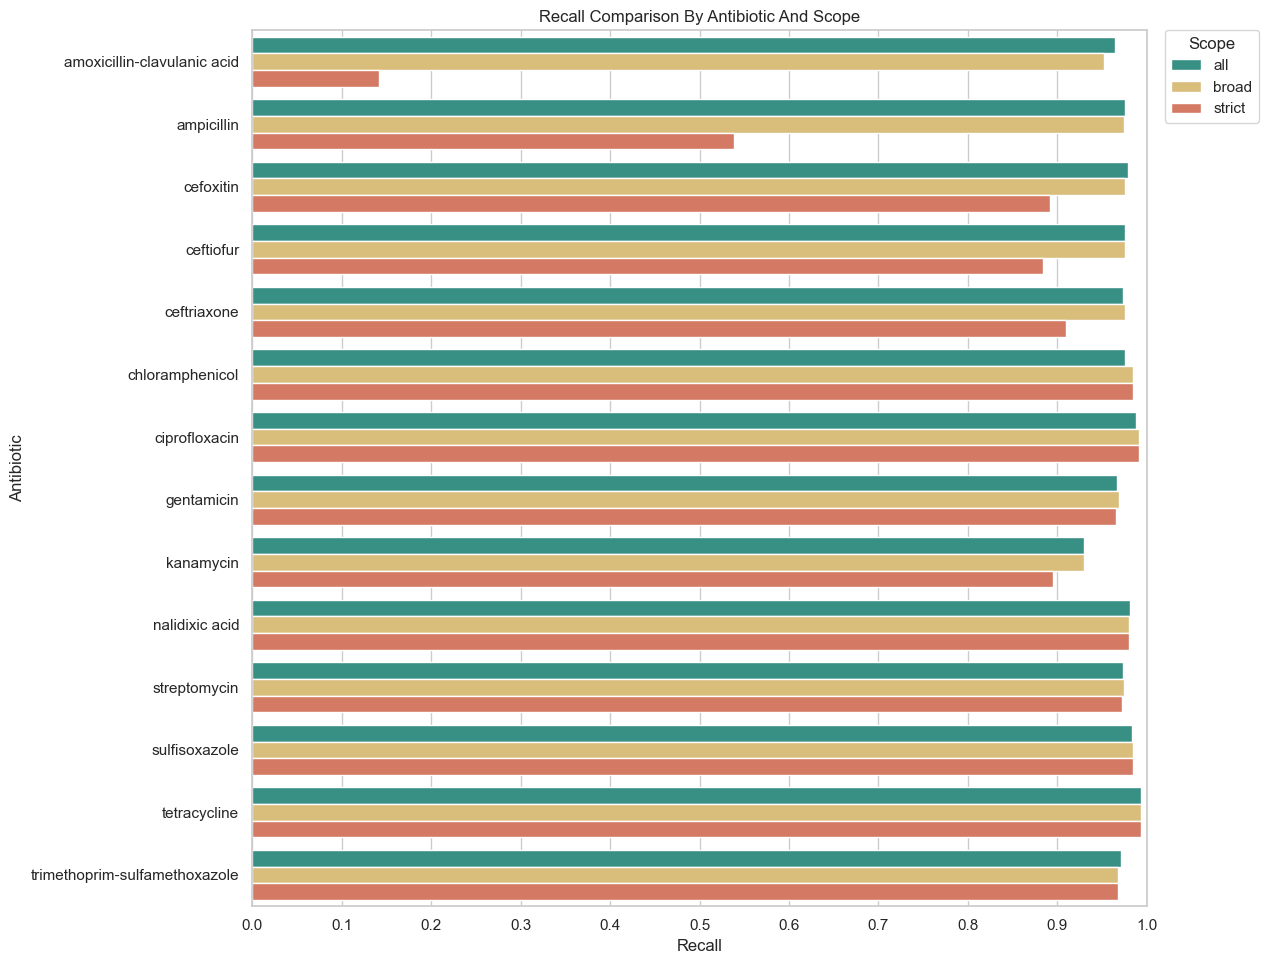
\includegraphics[width=\textwidth]{figures/recall_by_scope}
\caption{Recall by scope.}
\label{fig:recall-by-scope}
\end{subfigure}\hfill
\begin{subfigure}[t]{0.49\textwidth}
\centering
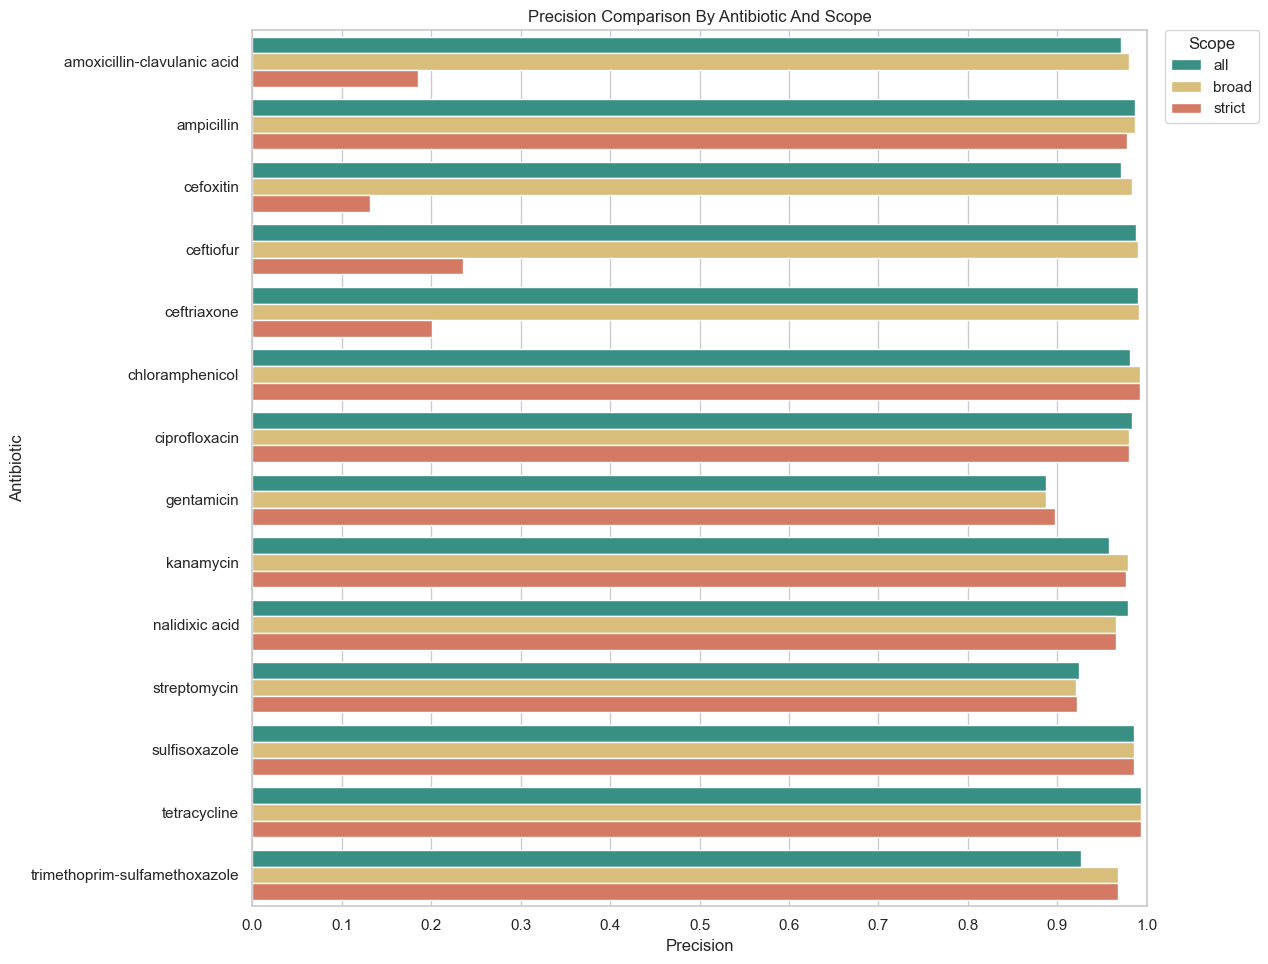
\includegraphics[width=\textwidth]{figures/precision_by_scope}
\caption{Precision by scope.}
\label{fig:precision-by-scope}
\end{subfigure}

\vspace{0.75em}

\begin{subfigure}[t]{0.82\textwidth}
\centering
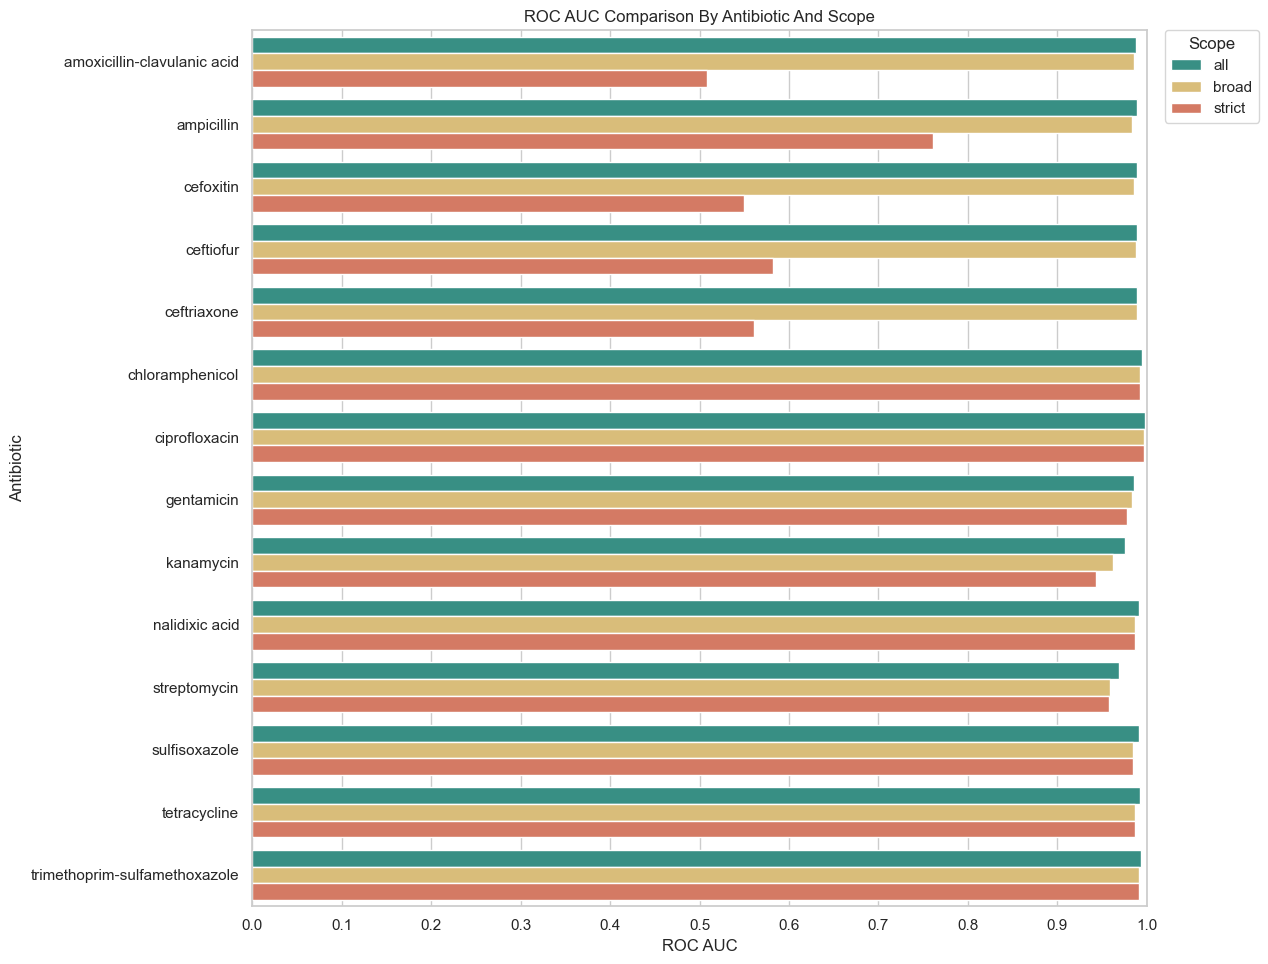
\includegraphics[width=\textwidth]{figures/roc_auc_by_scope}
\caption{ROC-AUC by scope.}
\label{fig:roc-auc-by-scope}
\end{subfigure}
\caption[Performance comparison across antibiotics and scopes.]{Performance comparison across antibiotics and determinant-connection scopes.}
\label{fig:scope-performance-comparison}
\end{figure}

Figure~\ref{fig:scope-performance-comparison} reveals the same underlying pattern from different angles. Recall highlights where broader evidence is needed to recover resistant isolates. Precision highlights whether a wide scope is overcalling resistance. ROC-AUC then shows whether the model is still separating resistant and susceptible isolates well across thresholds even when the exact operating point differs.

\subsection{Best scope by antibiotic}

Because this is an antibiotic-specific problem, average metrics do not tell the full story. Using the project's final priority ordering of recall first, precision second, and ROC-AUC third, the best-performing scope per antibiotic is summarized in Table~\ref{tab:best-scope-by-antibiotic}.

\begin{table}[H]
\centering
\caption{Best-performing scope by antibiotic under the final metric priority}
\label{tab:best-scope-by-antibiotic}
\small
\begin{tabular}{ll}
\toprule
Antibiotic & Best scope \\
\midrule
amoxicillin-clavulanic acid & all \\
ampicillin & all \\
cefoxitin & all \\
ceftiofur & broad \\
ceftriaxone & broad \\
chloramphenicol & strict \\
ciprofloxacin & strict \\
gentamicin & broad \\
kanamycin & broad \\
nalidixic acid & all \\
streptomycin & broad \\
sulfisoxazole & strict \\
tetracycline & all \\
trimethoprim-sulfamethoxazole & all \\
\bottomrule
\end{tabular}
\end{table}

The counts are also informative. \textit{All} wins on 6 antibiotics, \textit{broad} wins on 5, and \textit{strict} wins on 3. This reinforces the main interpretation that the widest scope is the strongest default overall, while narrower biologically constrained settings are still preferable for some antibiotics where direct mechanism specificity remains strong.

\section{Interpretation of Model Behavior}

\subsection{Rule-based versus machine-learning behavior}

The rule-based baselines are useful because they show when connected determinant evidence is already sufficient for direct phenotype inference and when learned combination becomes necessary.

For some antibiotics, the narrow direct rule is already very strong. Under the strict scope, ciprofloxacin reaches precision \(0.968\) and recall \(0.998\), chloramphenicol reaches precision \(0.990\) and recall \(0.988\), and nalidixic acid reaches precision \(0.953\) and recall \(0.989\). These antibiotics are exactly the cases where the retained determinant set already tracks the phenotype closely.

For other antibiotics, however, direct rules become too weak or too coarse. Under the strict rule baseline, ceftriaxone reaches recall only \(0.101\) and precision \(0.090\), while ceftiofur reaches recall \(0.133\) and precision \(0.102\). Under broad rule-based matching, ceftriaxone recall rises sharply to \(0.985\), but precision remains only \(0.489\). This is the clearest demonstration of the core trade-off: broader within-class evidence can recover resistant isolates, but a direct rule does not know how to combine or down-weight that evidence selectively.

Machine learning changes this balance substantially. For ceftriaxone, \textit{broad ML} achieves precision \(0.992\) and recall \(0.976\), while \textit{all ML} reaches precision \(0.990\) and recall \(0.974\). In other words, the learned models preserve the broad evidence needed for sensitivity, but avoid much of the precision collapse seen in broad rule-based inference. This pattern is one of the strongest arguments for the machine-learning stage in the final workflow.

\subsection{Zero-feature rows and coverage limits}

One of the clearest empirical signals in the project is the role of all-zero rows. In the rule-based setting, a zero-hit row means that no determinant connected to the target scope was found. In the machine-learning setting, the same situation appears as an all-zero feature vector.

The averages in Table~\ref{tab:method-average-metrics} show that \textit{strict} settings contain about \(4461\) zero rows on average, \textit{broad} settings contain about \(3790.5\), and \textit{all} contains none.

This explains much of the gap between \textit{strict} and the broader settings. A biologically conservative scope may be attractive conceptually, but if it leaves a large fraction of the valid phenotype cohort with no retained determinant evidence, both rule-based inference and machine learning start from a weak representation.

\subsection{Feature-importance interpretation}

Feature-importance scores help show whether the learned models are relying on biologically plausible determinants and how that behavior changes by scope.

\paragraph{Strict scope: direct mechanism alignment.}
For ciprofloxacin under \textit{strict}, the top-ranked features are dominated by quinolone-related mutations and genes, especially \texttt{gyrA\_D87Y}, \texttt{gyrA\_S83F}, \texttt{qnrB19}, and \texttt{qnrS} features. This matches the strong performance of \textit{strict} on ciprofloxacin and supports the interpretation that direct mutation-level evidence is already highly informative in this case.

\paragraph{Broad scope: cross-resistance evidence becomes useful.}
For ceftriaxone under \textit{broad}, the top-ranked features are led by beta-lactamase-related determinants such as \texttt{blaCTX-M-65} and \texttt{blaCMY-2}. This is exactly the biological pattern that motivated the broad setting: class-level cephalosporin and beta-lactam resistance signals are relevant even when narrow subclass matching would be too restrictive.

\paragraph{All scope: strongest coverage, but with leakage risk.}
The \textit{all} scope produces the strongest global default, but the feature-importance outputs also show why interpretability must be handled carefully. For amoxicillin-clavulanic acid under \textit{all}, top-ranked features still include plausible beta-lactamase-related signals such as \texttt{blaCMY-2}, but they also include determinants such as \texttt{ant(2'')-Ia} and quinolone-related \texttt{gyrA} mutation features. These are likely reflecting broader co-occurrence structure rather than direct mechanism-specific relevance to the target drug.

The same pattern appears in gentamicin and trimethoprim-sulfamethoxazole under \textit{all}. Important expected signals remain visible, but unrelated or only indirectly related determinants can also rise in the ranking. This does not invalidate the predictive benefit of \textit{all}; rather, it clarifies why \textit{all} should be described as a high-performance but less biologically constrained representation.

\subsection{Error analysis and failure modes}

The remaining errors follow three main patterns, and these patterns should be read by \emph{both} scope and method family. The labels \textit{strict} and \textit{broad} appear in both the rule-based and machine-learning settings, but they do not fail in exactly the same way.

\paragraph{Pattern 1: strict-scope sparsity affects both method families.}
The first pattern is the loss of useful evidence under the narrowest scope. In the \textit{strict rule-based} setting, this appears mainly as false negatives: ceftriaxone reaches recall only \(0.101\) and ceftiofur reaches \(0.133\). In \textit{strict ML}, the same sparse representation still causes serious instability, even though the model is no longer a direct rule. For the same two antibiotics, strict ML precision is only \(0.201\) for ceftriaxone and \(0.235\) for ceftiofur. The shared cause is the large number of zero-feature rows under the strict scope. The difference is that the rule-based model fails by directly missing resistant isolates, whereas the learned model fails because the retained representation is too weak for reliable separation.

\paragraph{Pattern 2: broad-scope overcalling is mainly a rule-based failure.}
The second pattern is scope-driven false positives under \textit{broad rule-based} inference. Here recall is recovered, but precision collapses because any within-class determinant hit is treated as sufficient evidence of resistance. Precision falls to \(0.489\) for ceftriaxone, \(0.455\) for ceftiofur, \(0.331\) for cefoxitin, and \(0.488\) for amoxicillin-clavulanic acid. Gentamicin and kanamycin are even more extreme, with broad rule-based precision \(0.218\) and \(0.281\), respectively. This pattern should not be confused with \textit{broad ML}. The learned broad-scope models use the same wider evidence pool, but they do not collapse in the same way because they can weight and combine determinants instead of treating every hit as equally decisive.

\paragraph{Pattern 3: some antibiotics remain hard even for the strongest ML setting.}
The third pattern belongs specifically to the learned models. Even under \textit{all ML}, where feature coverage is maximal, a few antibiotics remain visibly harder than the rest. Gentamicin, kanamycin, and trimethoprim-sulfamethoxazole have all-scope precisions \(0.887\), \(0.958\), and \(0.927\), respectively, despite strong ROC-AUC values. This suggests that the model is ranking isolates reasonably well but that the final decision boundary still mixes directly relevant determinants with broader co-occurrence signals. In practical terms, these are antibiotics for which prediction remains useful, but interpretation should be more cautious than for easier cases such as ciprofloxacin or chloramphenicol.

Taken together, the error analysis reinforces the central conclusion of the study. Errors are not random. Some are caused by overly narrow evidence under \textit{strict} scope, some are caused by overcalling in \textit{broad rule-based} inference, and some remain even after learned combination because determinant presence does not map cleanly to phenotype for every antibiotic.

\subsection{Main conclusions from the experiments}

The experimental results support the following conclusions:
\begin{enumerate}[label=\arabic*.]
    \item \textbf{The determinant-connection rule is a major scientific variable.} Performance changes substantially depending on whether evidence is connected narrowly, broadly, or without biological restriction.
    \item \textbf{Broad scope captures a meaningful cross-resistance signal.} It is the strongest biologically constrained alternative and often improves dramatically over strict matching for beta-lactam-related tasks.
    \item \textbf{All scope is the strongest global default for predictive performance.} Its main advantages are complete feature coverage and the best overall separability, but these come with a greater risk of co-occurrence leakage.
    \item \textbf{Strict scope remains valuable as a biological reference.} It is not the best universal choice, but it performs very well for antibiotics whose phenotype is tightly linked to narrow determinant signatures.
    \item \textbf{Machine learning adds most value when broad evidence must be combined selectively.} Direct rules can already be strong for some antibiotics, but they become too crude when broader within-class evidence is necessary.
\end{enumerate}

\section{Study Limitations}

This study predicts a binary resistant/susceptible phenotype rather than MIC, uses curated determinant resources rather than full pan-genome features, and has not yet performed external validation on an independent cohort. In addition, feature-importance analysis identifies strong predictive features rather than proving causal biological mechanisms. These limitations define the scope of the study clearly: it is a determinant-based bioinformatics analysis of AMR prediction behavior, not yet a full clinical deployment study.
